\documentclass{standalone}

% Plotting
\usepackage{tikz}
\usetikzlibrary{decorations.markings}
\usetikzlibrary{calc}
% quantikz breaks tikz-cd, see https://tex.stackexchange.com/questions/618330/quantikz-breaks-spacing-in-tikz-matrices-tikz-cd
%\usetikzlibrary{quantikz}
\usetikzlibrary{cd}
\usepackage{pgfplots}

\usepackage{simpler-wick}
\usepackage{physics}

\usepackage{amsmath}
\usepackage{mathtools}

\begin{document}
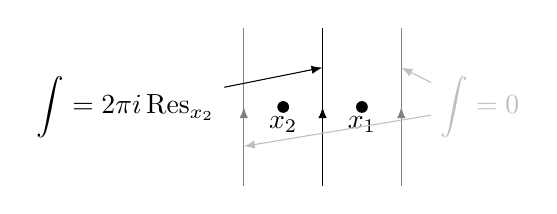
\begin{tikzpicture}
    \node (x2) at (0,0) [circle,fill,inner sep=1.5pt]{};
    \node (x1) at (1,0) [circle,fill,inner sep=1.5pt]{};

    \draw (x1) node[below] {$x_1$};
    \draw (x2) node[below] {$x_2$};
    

    \begin{scope}[,decoration={
        markings,
        mark=at position 0.5 with {\arrow{latex}}}]
        \draw[gray,postaction={decorate}] (-0.5, -1) -- (-0.5, 1);
        \draw[postaction={decorate}] (0.5, -1) -- (0.5, 1);
        \draw[gray,postaction={decorate}] (1.5, -1) -- (1.5, 1);
    \end{scope}

    \draw[lightgray] (2.5,0) node (int0) {$\displaystyle \int = 0$};
    \draw[lightgray,-latex] (int0) -- (-0.5,-0.5);
    \draw[lightgray,-latex] (int0) -- (1.5,0.5);

    \draw (-2,0) node (intres) {$\displaystyle \int = 2\pi i \operatorname{Res}_{x_2}$};
    \draw[-latex] (intres) -- (0.5, 0.5);
\end{tikzpicture}
\end{document}